\documentclass[xetex,mathserif,serif]{beamer}
\usepackage{polyglossia}
\setdefaultlanguage[babelshorthands=true]{russian}
\usepackage{minted}
\usepackage{tabu}

\useoutertheme{infolines}

\usepackage{fontspec}
\setmainfont{FreeSans}
\newfontfamily{\russianfonttt}{FreeSans}

\definecolor{links}{HTML}{2A1B81}
\hypersetup{colorlinks,linkcolor=,urlcolor=links}

\tabulinesep=0.7mm

\title{Пример архитектуры --- Bash}
\author[Юрий Литвинов]{Юрий Литвинов \newline \textcolor{gray}{\small\texttt{yurii.litvinov@gmail.com}}}

\date{22.01.2020г}

\begin{document}
	
	\frame{\titlepage}

	\section{Enterprise Fizz-Buzz}

	\begin{frame}
		\frametitle{Enterprise Fizz-Buzz}
		Задача:

		Для чисел от 1 до 100:
		\begin{itemize}
			\item если число делится на 3, вывести ``Fizz''
			\item если число делится на 5, вывести ``Buzz''
			\item если число делится и на 3, и на 5, вывести ``FizzBuzz''
			\item во всех остальных случаях вывести само число
		\end{itemize}

		Решение:

		\url{https://github.com/EnterpriseQualityCoding/FizzBuzzEnterpriseEdition}
	\end{frame}

	\begin{frame}
		\frametitle{Структура системы}
		\begin{center}
			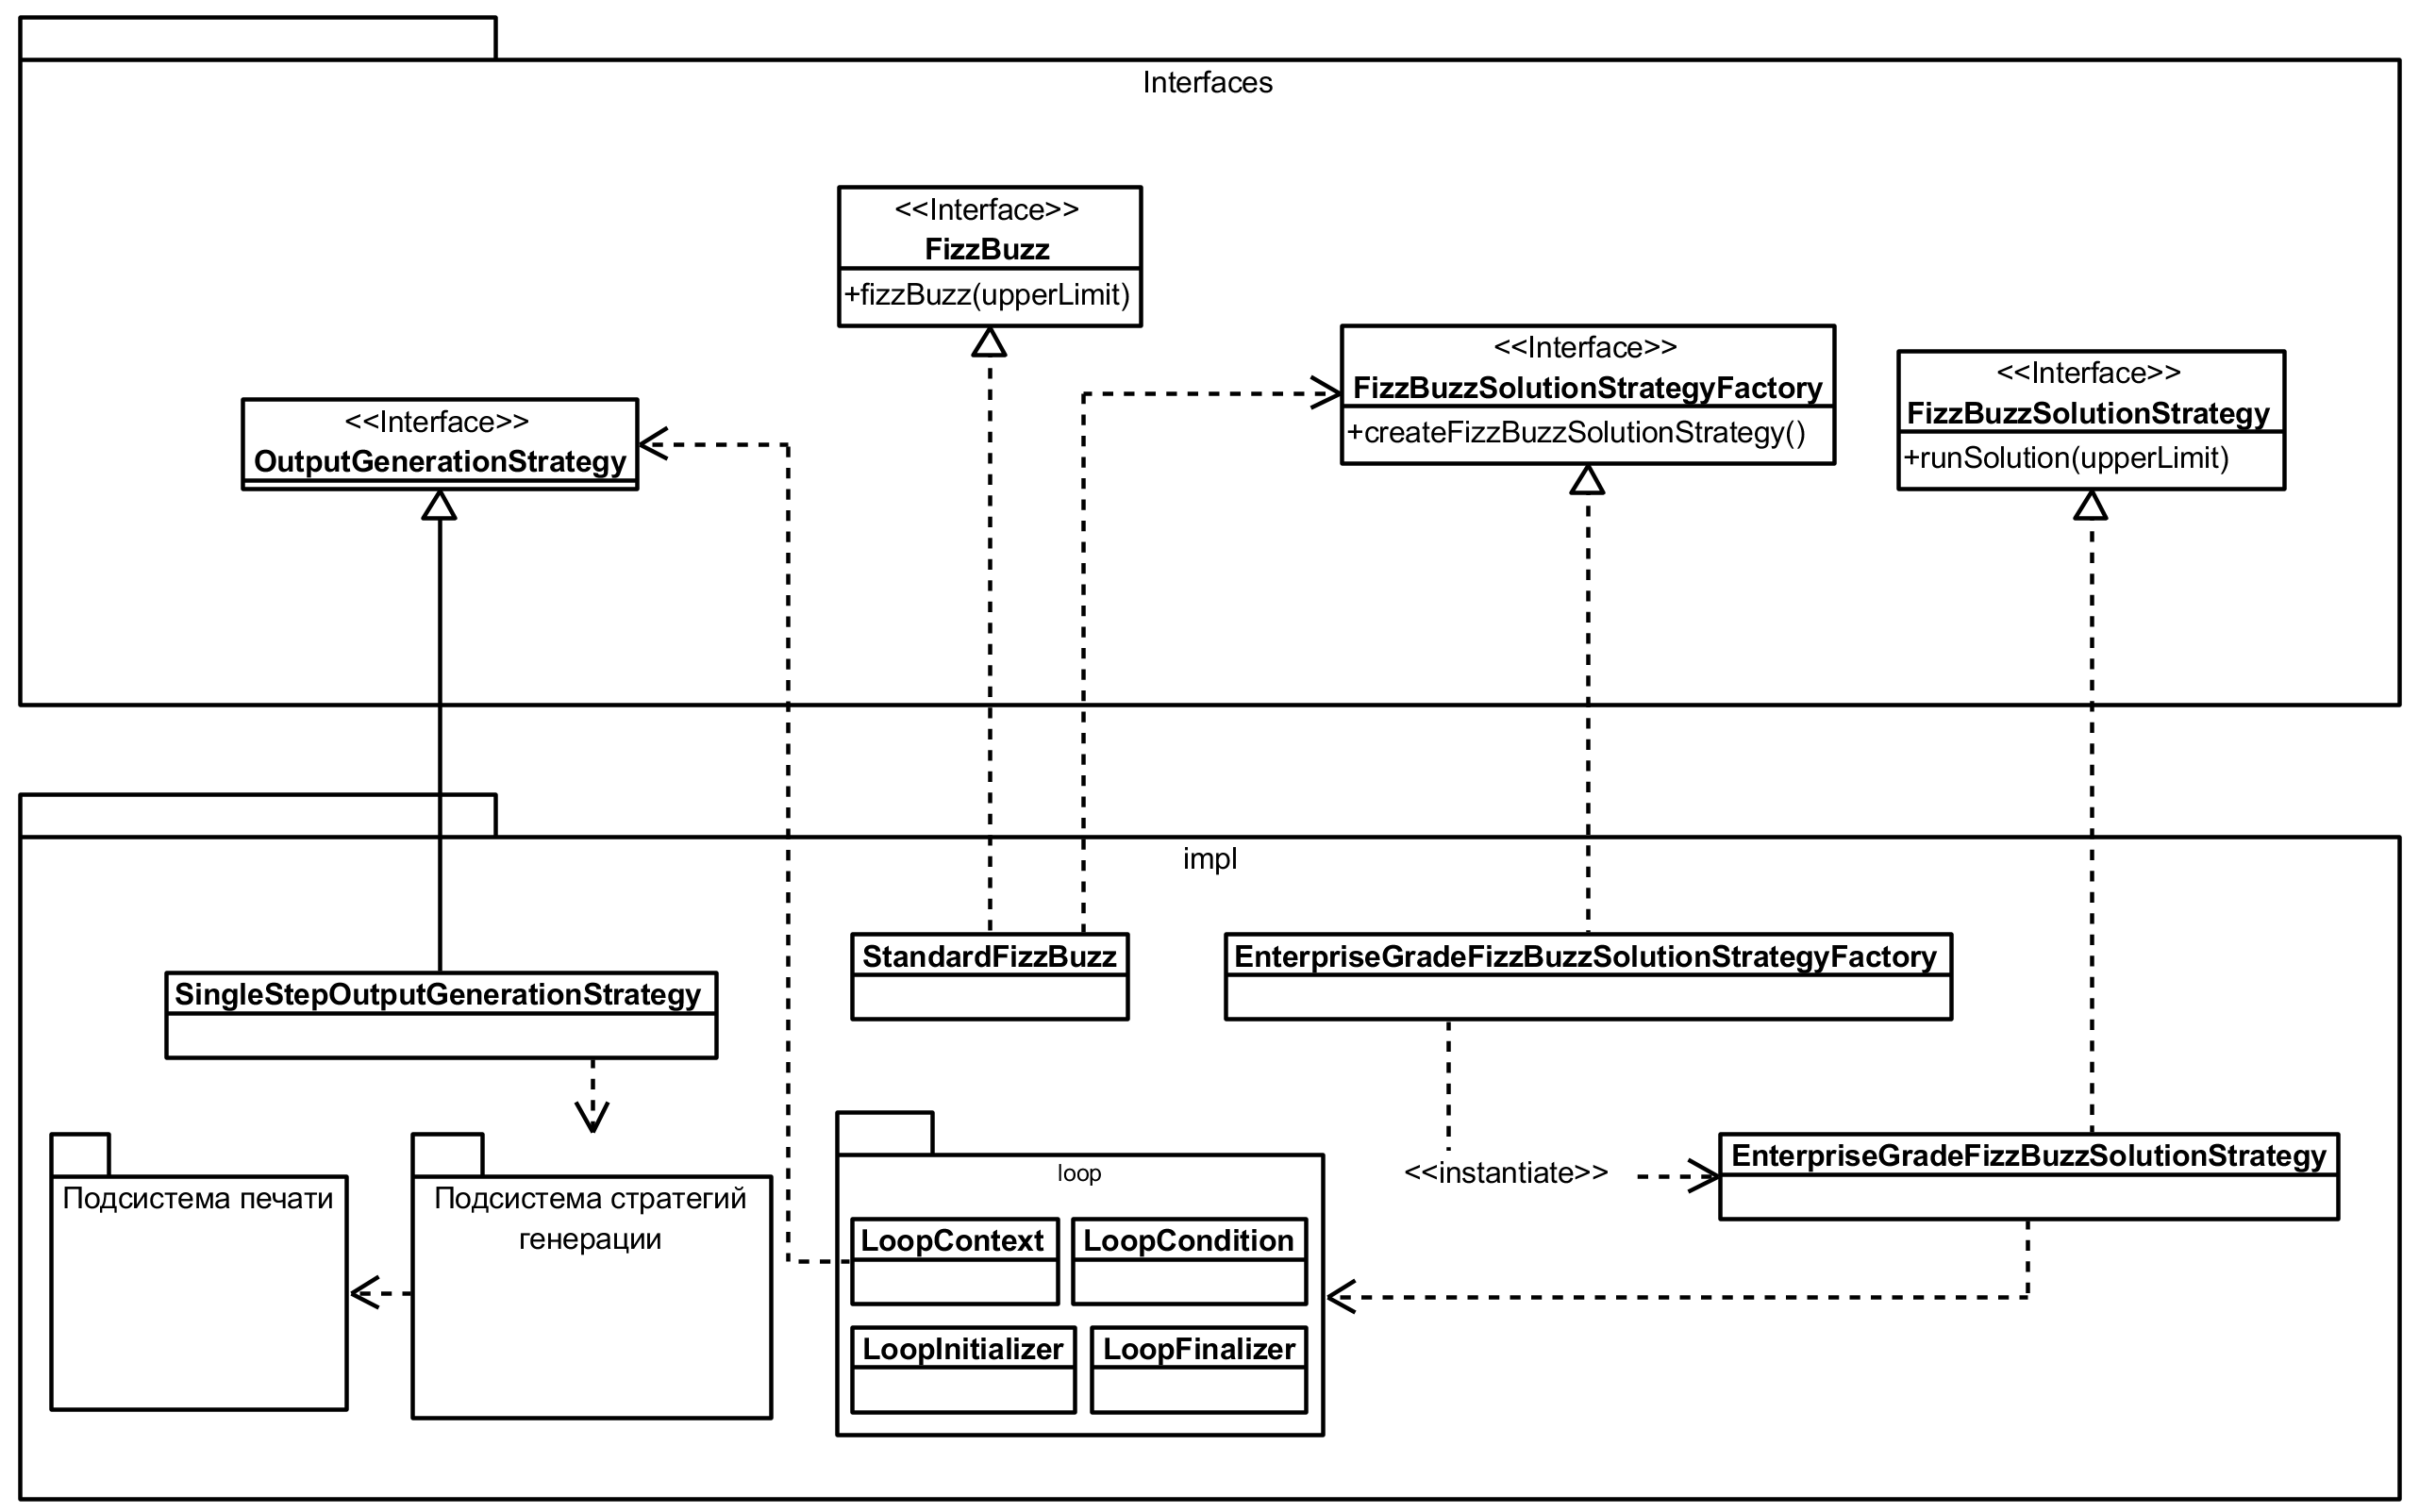
\includegraphics[width=\textwidth]{fizzBuzzArchitecture.png}
		\end{center}
	\end{frame}

	\begin{frame}
		\frametitle{Хорошие идеи}
		\begin{itemize}
			\item Separation of Concerns
			\item Dependency Inversion
			\item Dependency Injection
			\begin{itemize}
				\item Spring Framework
			\end{itemize}
			\item Паттерны ``Фабрика'', ``Стратегия'', ``Посетитель'', ``Адаптер'', что-то вроде паттернов ``Спецификация'' и ``Цепочка ответственности''
		\end{itemize}
	\end{frame}

	\begin{frame}
		\frametitle{Плохие идеи}
		\begin{itemize}
			\item Не выполняется принцип Keep It Simple Stupid
			\begin{itemize}
				\item Неправильно говорить ``строк кода написано'', правильно --- ``строк кода израсходовано''
			\end{itemize}
			\item ``Синтаксическое'' разделение на пакеты, а не ``семантическое''
			\begin{itemize}
				\item Отсуствие модульности, антипаттерн ``Big Ball of Mud''
			\end{itemize}
			\item Хардкод основных параметров вычисления
			\item Нет юнит-тестов, только интеграционные; нет логирования
			\item 1662 строки кода, очень мало комментариев (несмотря на недавно принятый пуллреквест ``Serious Documentation'')
			\begin{itemize}
				\item Отсутствие архитектурного описания
			\end{itemize}
		\end{itemize}
	\end{frame}

	\section{Bash}

	\begin{frame}
		\frametitle{Bash}
		\begin{itemize}
			\item Примерно 70К строк кода
			\item Исходный автор --- Brian Fox, maintainer --- Chet Ramey
			\item Первый релиз --- 1989
			\item Написан на C
			\item Архитектурное описание --- глава в \textit{The Architecture of Open Source Applications}, написанная Chet Ramey
		\end{itemize}
	\end{frame}

	\begin{frame}
		\frametitle{Архитектура Bash}
		\begin{center}
			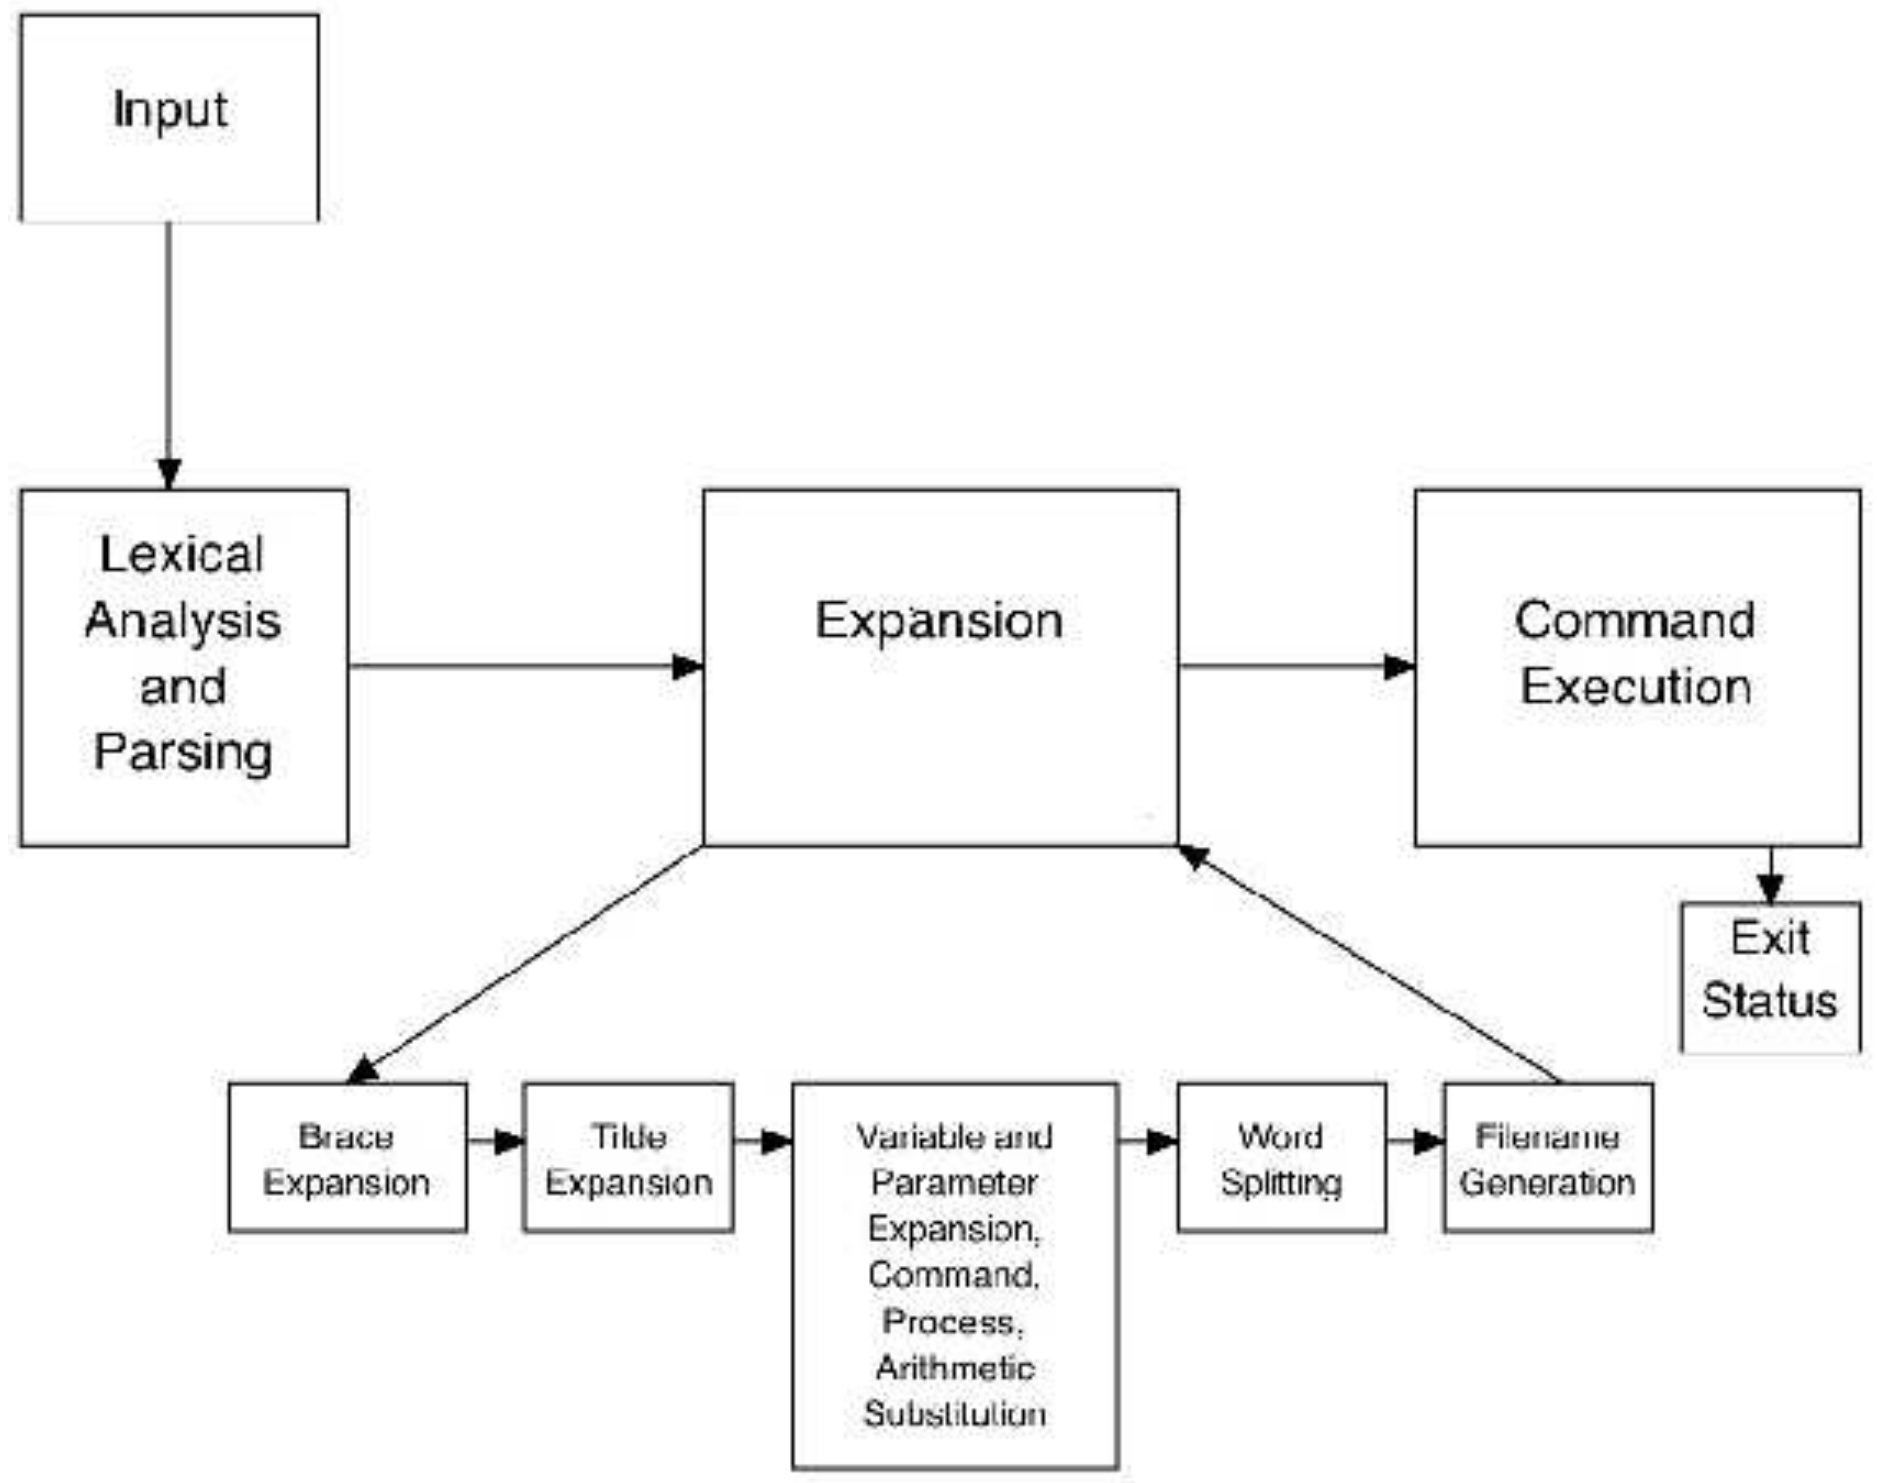
\includegraphics[width=0.7\textwidth]{bashArchitecture.png}
		\end{center}
	\end{frame}

	\begin{frame}[fragile]
		\frametitle{Основные структуры данных}
		\begin{minted}{c}
typedef struct word_desc {
    char *word; /* Zero terminated string. */
    int flags; /* Flags associated with this word. */
} WORD_DESC;
		\end{minted}

		\vspace{3mm}

		\begin{minted}{c}
typedef struct word_list {
    struct word_list *next;
    WORD_DESC *word;
} WORD_LIST;
		\end{minted}
	\end{frame}

	\begin{frame}
		\frametitle{Ввод с консоли}
		\begin{itemize}
			\item Библиотека Readline
			\begin{itemize}
				\item независимая библиотека, но пишется в основном для Bash
			\end{itemize}
			\item Цикл read/dispatch/execute/redisplay
			\item Dispatch table (или Keymap)
			\item Буфер редактирования, хитрый механизм расчёта действий для отображения
			\item Хранит все данные как 8-битные символы, но знает про Unicode
		\end{itemize}
	\end{frame}

	\begin{frame}[fragile]
		\frametitle{Синтаксический разбор}
		\begin{itemize}
			\item Зависимый от контекста лексический анализ
				\begin{minted}{sh}
for for in for; do for=for; done; echo $for
				\end{minted}
			\item Использует lex + bison
			\item Подстановка alias-ов выполняется лексером
			\item Сохранение и восстановление состояния парсера
		\end{itemize}
	\end{frame}

	\begin{frame}[fragile]
		\frametitle{Подстановки}
		\begin{minted}{sh}
${parameter:-word}
		\end{minted}

раскрывается в \textit{parameter}, если он установлен, и в \textit{word}, если нет

		\begin{minted}{sh}
pre{one,two,three}post
		\end{minted}

раскрывается в 

		\begin{minted}{sh}
preonepost pretwopost prethreepost
		\end{minted}

		Ещё бывает подстановка тильды и арифметическая подстановка, сопоставление шаблона
	\end{frame}

	\begin{frame}[fragile]
		\frametitle{Исполнение команд}
		\begin{itemize}
			\item Встроенные и внешние команды, обрабатываются единообразно
			\item Перенаправление ввода-вывода, отмена перенаправления
			\item Принимают набор слов
			\begin{itemize}
				\item Иногда обрабатывают по-особому, например, присваивание в \textit{export}
			\end{itemize}
			\item Присваивание --- тоже команда, но особая
			\item Перед запуском внешней команды --- поиск в PATH, кеширование результатов
			\item Job control, foreground и background
		\end{itemize}
	\end{frame}

	\begin{frame}[fragile]
		\frametitle{Lessons Learned}
		\begin{itemize}
			\item Комментарии к коммитам со ссылками на багрепорты с шагами воспроизведения
			\item Хороший набор тестов, в Bash их тысячи
			\item Стандарты, как внешние на функциональность шелла, так и на код
			\item Пользовательская документация
			\item Переиспользование
		\end{itemize}
	\end{frame}

	\section{Bash, на самом деле}

	\begin{frame}
		\frametitle{Архитектура Bash, на самом деле}
		\begin{itemize}
			\item J. Garcia et al., \textit{Obtaining Ground-Truth Software Architectures}
			\item 1 аспирант, 80 часов работы
			\item Верификация от Chet Ramey
			\item 70К строк кода, 200 файлов, 25 компонент
			\begin{itemize}
				\item 16 --- ядро, 9 --- утилиты
			\end{itemize}
			\item Структура папок почти не соответствует выделенным компонентам
		\end{itemize}
	\end{frame}

	\begin{frame}
		\frametitle{Архитектура Bash, на самом деле}
		\begin{center}
			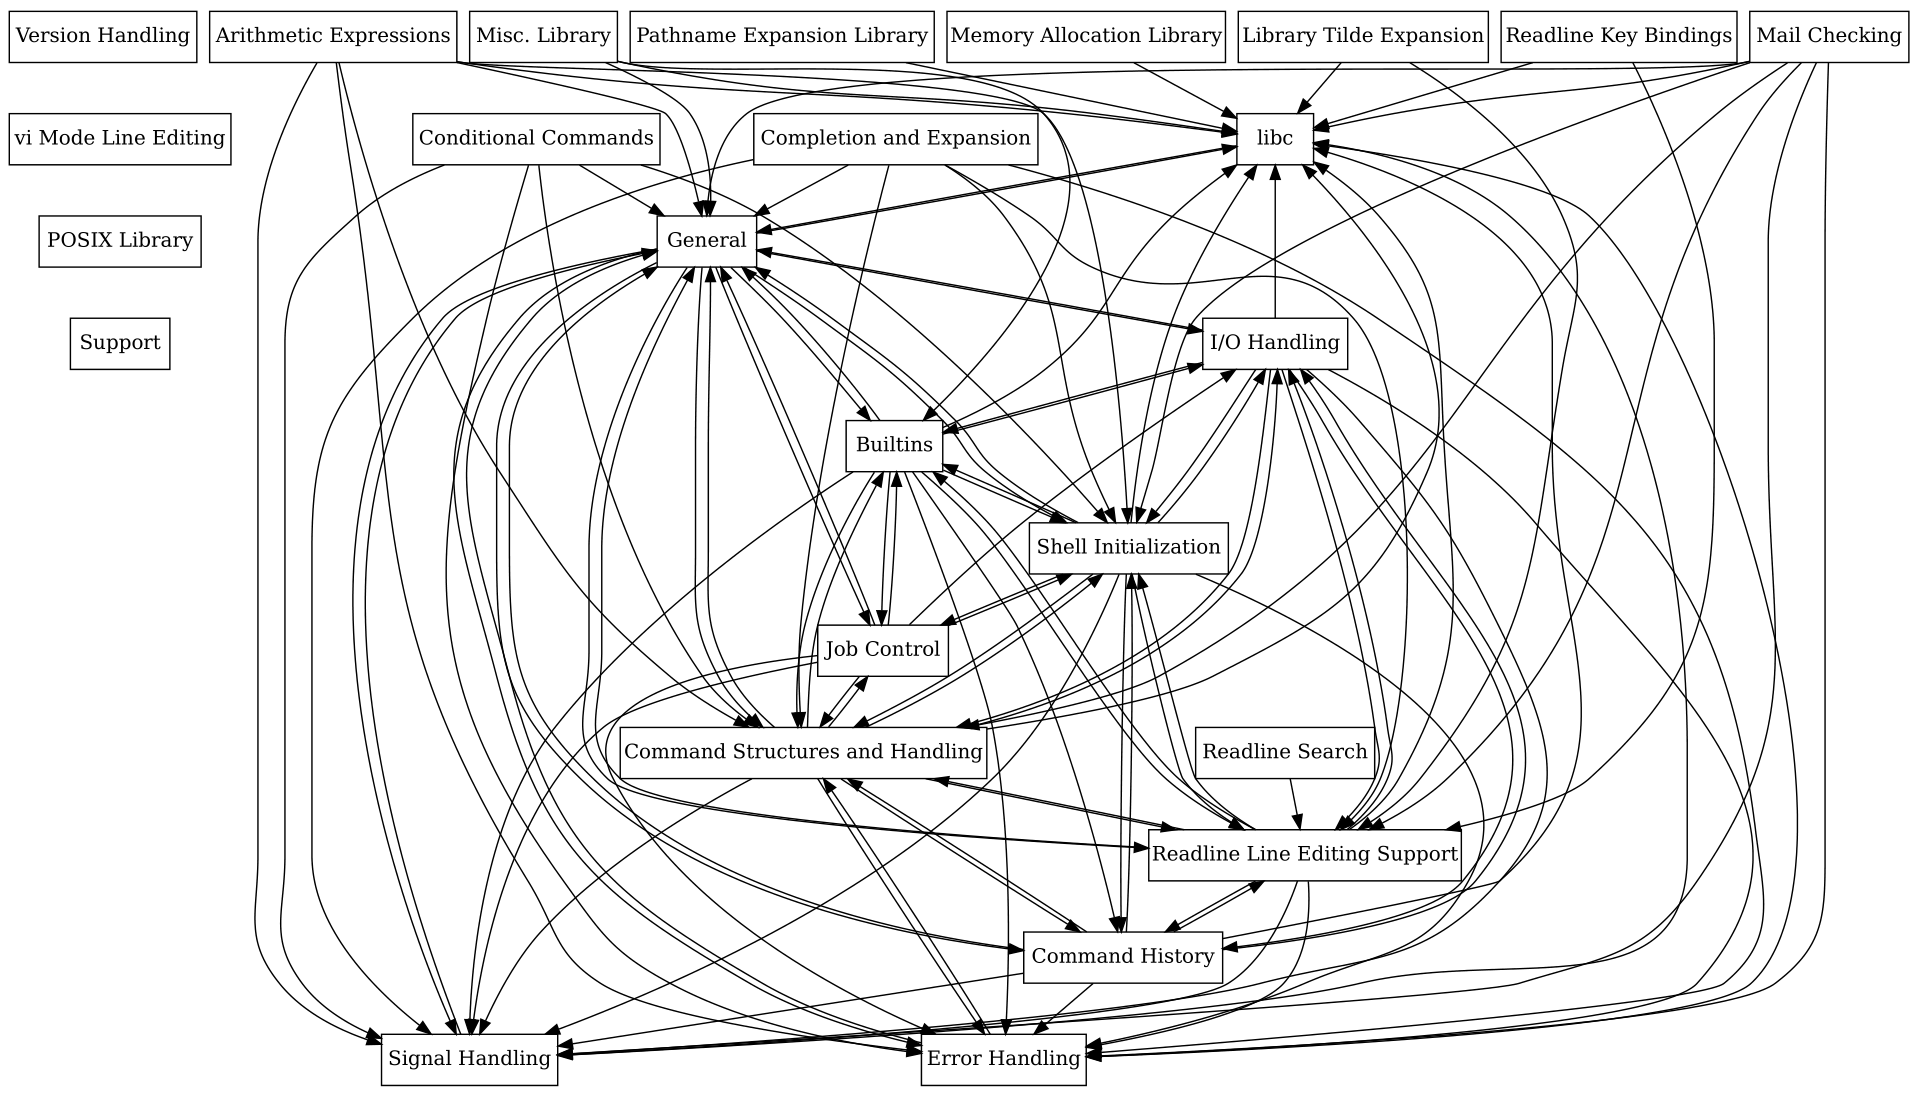
\includegraphics[width=\textwidth]{bashRealArchitecture.png}
		\end{center}
	\end{frame}

	\begin{frame}
		\frametitle{Результаты анализа кода}
		\begin{center}
			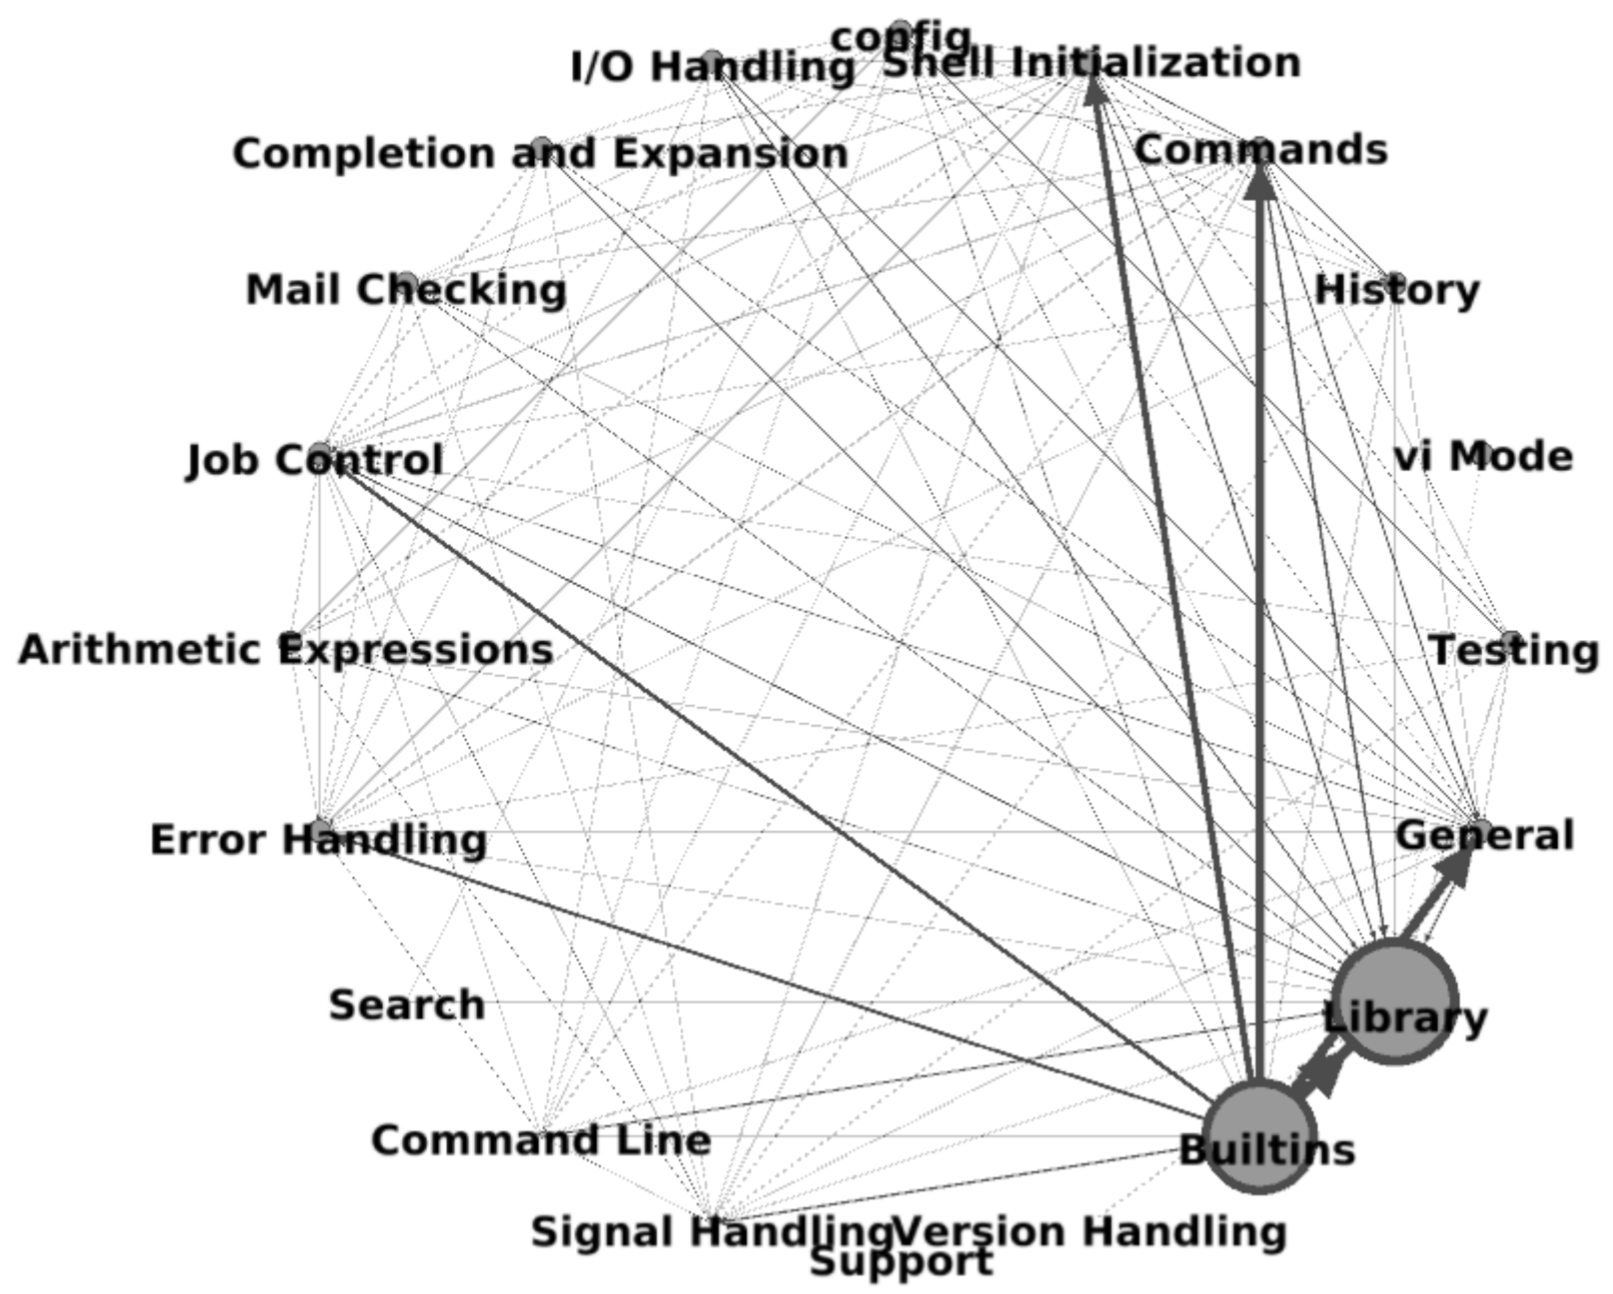
\includegraphics[width=0.7\textwidth]{bashAutomaticRecoveryArchitecture.png}
		\end{center}
	\end{frame}

	\begin{frame}
		\frametitle{Сравним с исходной}
		\begin{center}
			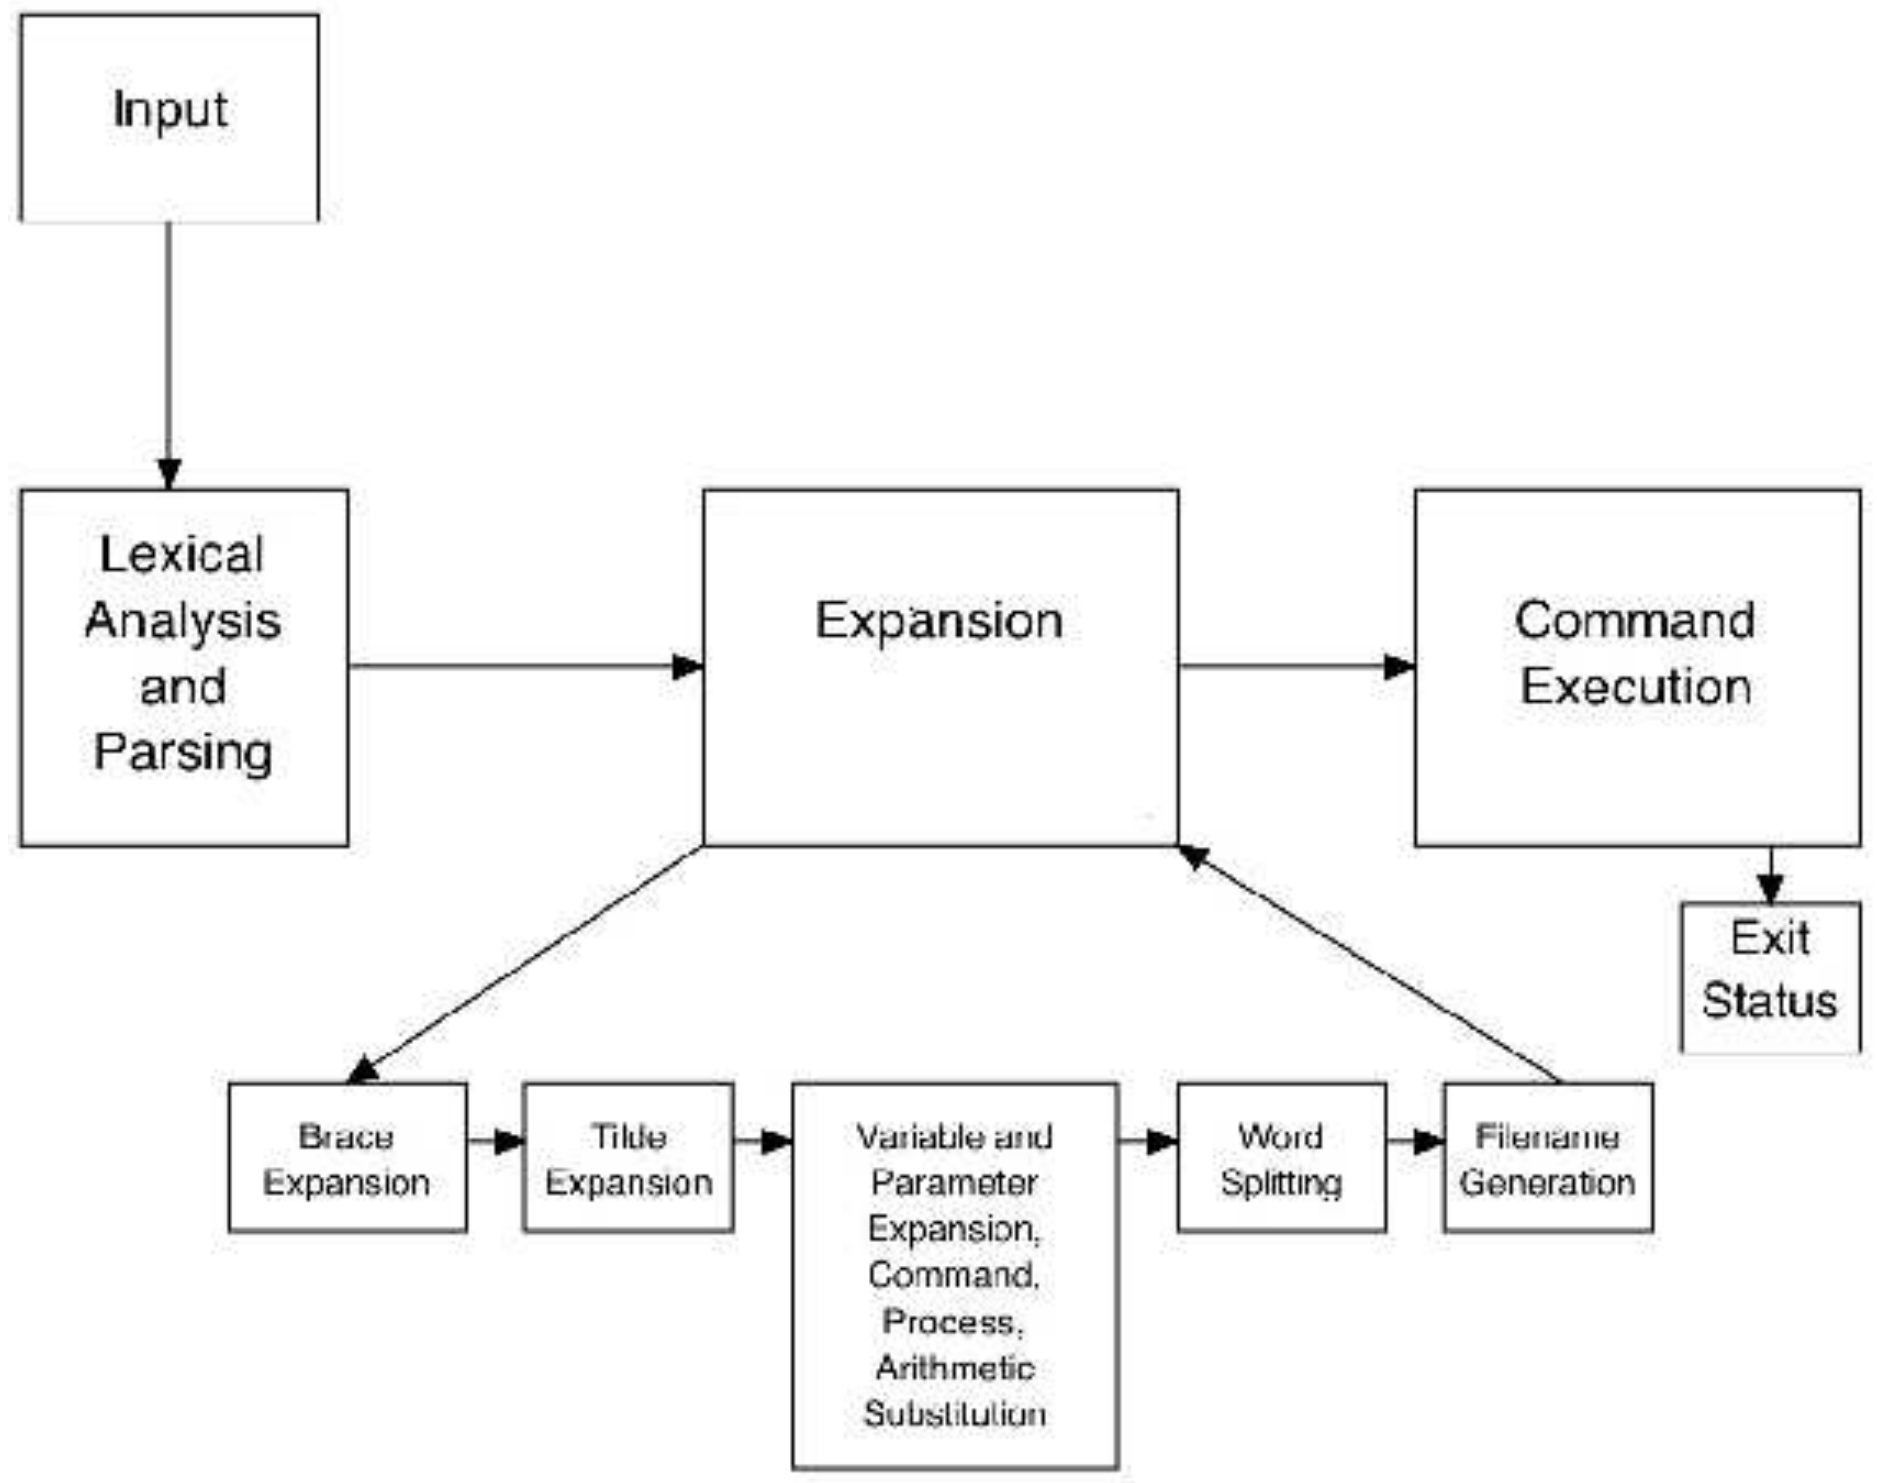
\includegraphics[width=0.7\textwidth]{bashArchitecture.png}
		\end{center}
	\end{frame}

	\begin{frame}
		\frametitle{Job Control}
		\begin{center}
			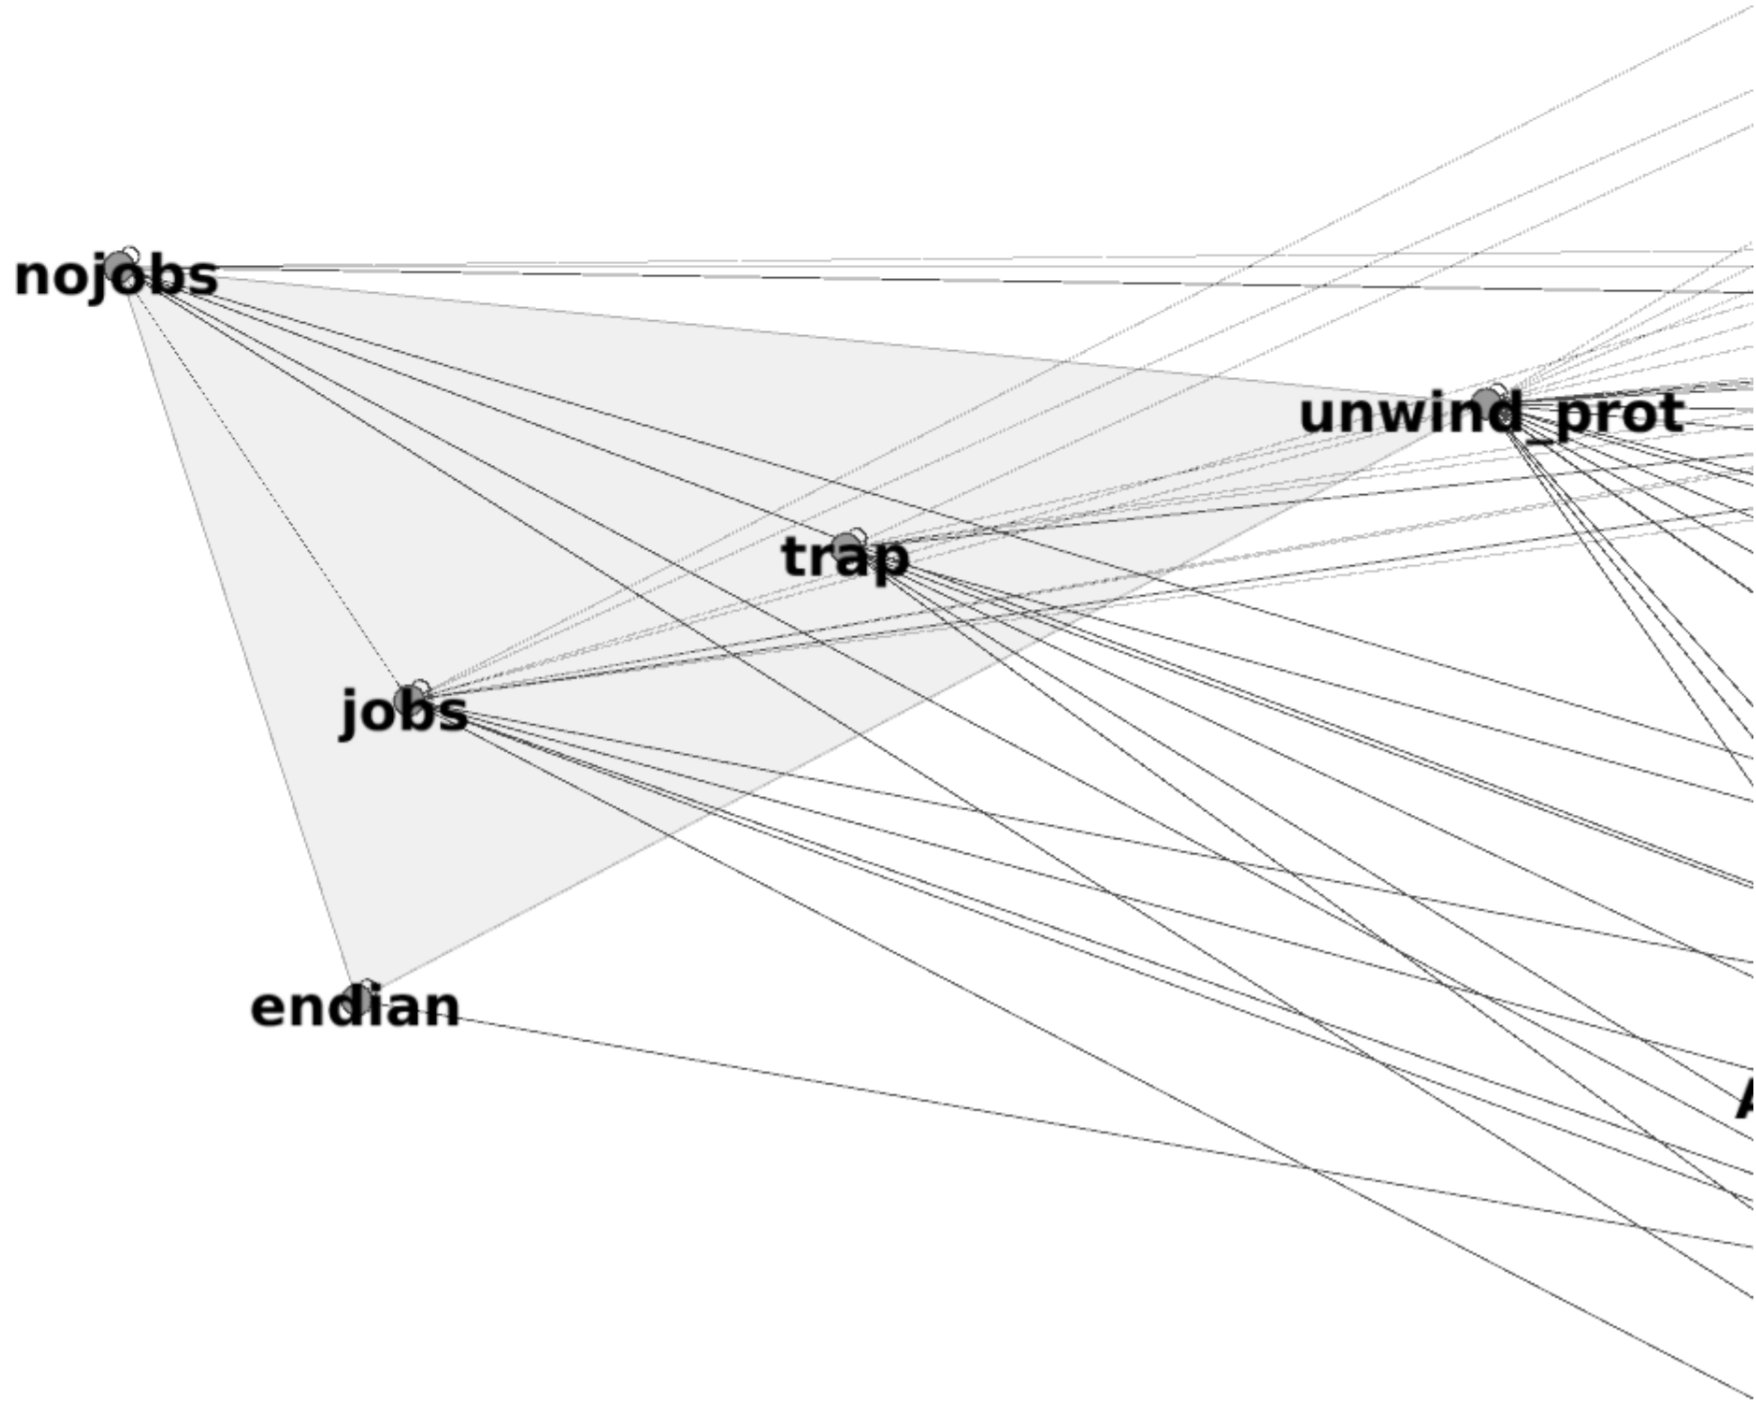
\includegraphics[width=0.7\textwidth]{bashJobControl.png}
		\end{center}
	\end{frame}

	\begin{frame}
		\frametitle{Commands}
		\begin{center}
			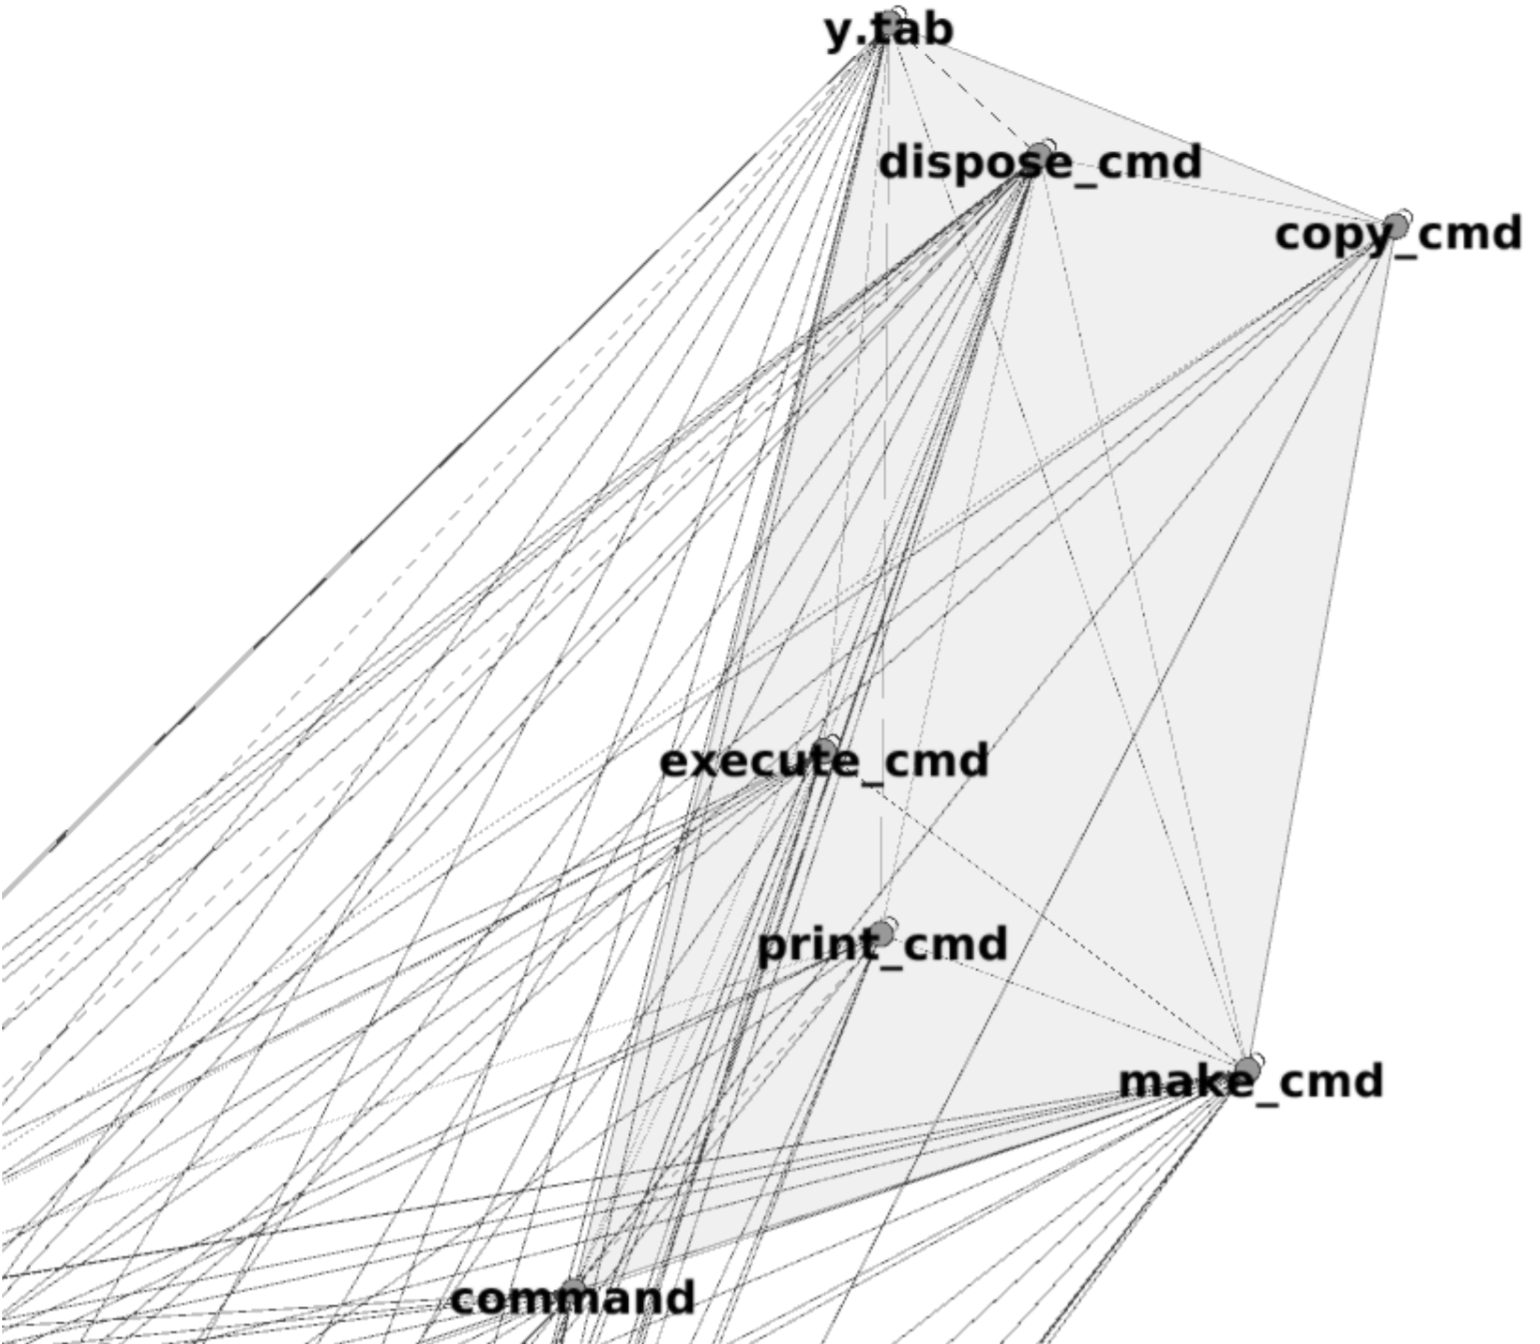
\includegraphics[width=0.7\textwidth]{bashCommands.png}
		\end{center}
	\end{frame}

	\section{Grep}

	\begin{frame}
		\frametitle{Grep}
		\framesubtitle{Следующая задача}
		Реализовать команду grep, 
		\begin{itemize}
			\item поддерживающую ключи
			\begin{itemize}
				\item \textit{-i} (нечувствительность к регистру)
				\item \textit{-w} (поиск только слов целиком)
				\item \textit{-A n} (распечатать n строк после строки с совпадением)
			\end{itemize}
			\item поддерживающую регулярные выражения в строке поиска
			\item использующую одну из библиотек для разбора аргументов командной строки
		\end{itemize}
	\end{frame}

	\begin{frame}[fragile]
		\frametitle{Примеры}
		\begin{minted}{bash}
> grep plugin build.gradle
    apply plugin: 'java'
    apply plugin: 'idea'
> cat build.gradle | grep plugin
    apply plugin: 'java'
    apply plugin: 'idea'
> grep -A 2 plugin build.gradle
    apply plugin: 'java'
    apply plugin: 'idea'
    group = 'ru.example'
    version = '1.0'
		\end{minted}
\end{frame}

	\begin{frame}
		\frametitle{Замечания}
		\begin{itemize}
			\item Ожидается обоснование выбора библиотеки для работы с аргументами
			\begin{itemize}
				\item Какие библиотеки были рассмотрены
				\item Почему выбрана именно та, что выбрана
				\begin{itemize}
					\item кратко описать текстом
				\end{itemize}
			\end{itemize}
			\item Сдавать как новый пуллреквест из новой ветки на базе предыдущей
		\end{itemize}
	\end{frame}

\end{document}
